\subsection{Weitere motorische Kerngebiete}
\subsubsection{Nucleus ventralis anterolateralis} \index{Nucleus! ventralis anterolateralis} \label{subsubsec:ncl_anterolateralis}
Der Nucleus ventralis anterolateralis ist ein Kerngebiet innerhalb des Thalamus, welches eine wichtige Funktion bei der Bewegungskoordination einnimmt. Dieser Bereich setzt sich aus zwei Teilgebieten zusammen, dem \textbf{Nucleus ventralis anterior} (VA) und dem \textbf{Nucleus ventralis lateralis} (VL) \textsuperscript{\cite[Kap.~8]{trepel2011neuroanatomie}}. Der ventrale laterale Kern bekommt Input aus dem  Globus pallidus und der Substantia nigra der ipsilateralen Seite, sowie aus dem contralateralen Nucleus dentatus des Cerebellums. Innerhalb des ventralen lateralen Bereichs lassen sich drei weitere Bereiche abgrenzen: der \textit{Pars oralis} (VLo), der \textit{Pars medialis} (VLm) und der \textit{Pars caudalis} (VLc). Die Afferenzen des Pallidums und der Substantia nigra enden im VLo und VLm, während die aus dem Kleinhirn zu dem Bereich des VLc projizieren. Auch das ventrale anteriore Kerngebiet lässt sich weiter unterteilen, in einen größeren Hauptbereich (\textbf{VApc}) und einen kleineren magnozellulären Bereich (\textbf{VAmc}). Afferenzen in dieser Region stammen auch aus dem Pallidum und der Substantia nigra. Der VApc erhält dabei Input aus dem inneren Teilbereich des Globus pallidus. Der VAmc erhält seine Afferenzen aus der Substantia nigra pars reticulata. Alle Bereiche des Nucleus ventralis anterolateralis besitzen eine reziproke Verbindung zu den motorischen Arealen des frontalen Cortex. Dabei ist die Verknüpfung zwischen dem VA und den prämotorischen und supplementärmotorischen Bereichen stärker. Der VL besitzt hauptsächlich Verbindungen zum primären Motorcortex \textsuperscript{\cite[Kap.~12]{crossman2014neuroanatomy}}. Damit übernimmt diese Kerngruppe eine essentielle Stellung innerhalb der motorischen Regulation, da hier die Information aus den Basalganglia und dem Kleinhirn zusammmenlaufen und diese Areale in Verbindung mit den motorischen Arealen des Großhirn wesentlich für das Entstehen und die Koordination der Willkürbewegung zuständig sind \textsuperscript{\cite[Kap.~8]{trepel2011neuroanatomie}}. In der Ratte können die Teilbereiche VA und VL nicht voneinander abgegrenzt werden, weshalb sie als \textbf{ventral-anteriorer/ventral-lateraler} (VAL) \textbf{Komplex} zusammengefasst werden \textsuperscript{\cite[Kap.~16]{paxinos2014rat}}.     

\subsubsection{Nuclei olivares inferiores} \index{Nuclei! olivares inferiores} \index{Olive! untere Olive} \label{subsubsec:untere_olive}
Der Kernkomplex der \textbf{Nuclei olivares inferiores} spielt ebenfalls eine wichtige Rolle in der Bewegungskoordination. Er ist innerhalb der Medulla oblongata lateral des Pyramidentrakts lokalisiert. Innerhalb dieses Komplexes lassen sich drei einzelne Kerngebiete unterscheiden. Der \textbf{Nucleus olivaris principalis} nimmt den größten Bereich ein und bildet damit den Hauptkern der Struktur. Daneben befinden sich zwei kleinere sogenannte Nebenoliven, mit dem \textbf{Nucleus olivaris accessorius medialis} und \textbf{Nucleus olivaris accessorius posterior}. Eingehende Informationen zu all diesen Kerngebieten stammen vor allem aus wichtigen motorischen Zentren. Besonders wichtig dabei sind die Projektionen aus dem Rückenmark, aus dem Nucleus ruber des Mittelhirns und aus dem motorischen Cortex des Großhirns. Der Input wird dann gesammelt in das Kleinhirn über den \textit{Tractus olivocerebellaris} gesendet. Dieser Faserstrang kreuzt auf die contralaterale Seite des Hirnstamms und verläuft über den Pedunculus cerebellaris inferior weiter in die Kleinhirnhälfte der Gegenseite. Die Fasern enden als Kletterfasern (siehe Kap.~\ref{sub:kleinhirn}) in der Kleinhirnrinde. Die Axone des Hauptkernes Ncl. olivaris principalis enden vorwiegend in der Kleinhirnhemisphäre, die efferenten Fasern der Nebenoliven ziehen zur Intermediärzone und zum Kleinhirnwurm hin. Damit stellen die Nuclei olivaris inferior ein wichtiges Verbindungsstück in der Bewegungskontrolle dar \textsuperscript{\cite[Kap.~5]{trepel2011neuroanatomie}}.  

\begin{figure}[H]
    \centering
    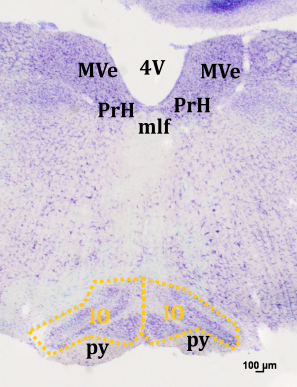
\includegraphics[width=0.4\textwidth]{pictures/Bilder_Laura/untere_olive_N04_4.png}
    \caption[Nuclei olivares inferiores]{\textbf{Nuclei olivares inferiores.} Der Kernkomplex der Nuclei olivares inferiores (IO) ist innerhalb der Medulla lateral zum Pyramidentrakt (py) lokalisiert. Dorsal zu erkennen sind der vierte Ventrikel (4V), der Nucleus vestibularis medialis (MVe), der Nucleus prepositus hypoglossi (PrH) und der Fasciculus longitudinalis medialis (mlf). Nissl-Färbung (N04-4).}
    \label{fig:untere_olive}
\end{figure}
